
\documentclass[12pt]{amsart}

\usepackage[utf8]{inputenc}
\usepackage[T1]{fontenc}
\usepackage{lmodern}
\usepackage[ngerman]{babel}
\usepackage{graphicx}
\usepackage{paralist}

\usepackage{Macros}

\usepackage{geometry} % see geometry.pdf on how to lay out the page. There's lots.
\geometry{a4paper} % or letter or a5paper or ... etc
% \geometry{landscape} % rotated page geometry

\title{Hausaufgabe 4 - Blatt 11 \& 12}
\author{Sarah Köhler und Matthias Loibl}
\date{} % delete this line to display the current date

%%% BEGIN DOCUMENT
\begin{document}

\maketitle
%\tableofcontents

%\section*{Blatt 11}

\section*{Aufgabe 1: Verbände}
\subsection*{a)}

\begin{figure}[h!]
\begin{center}
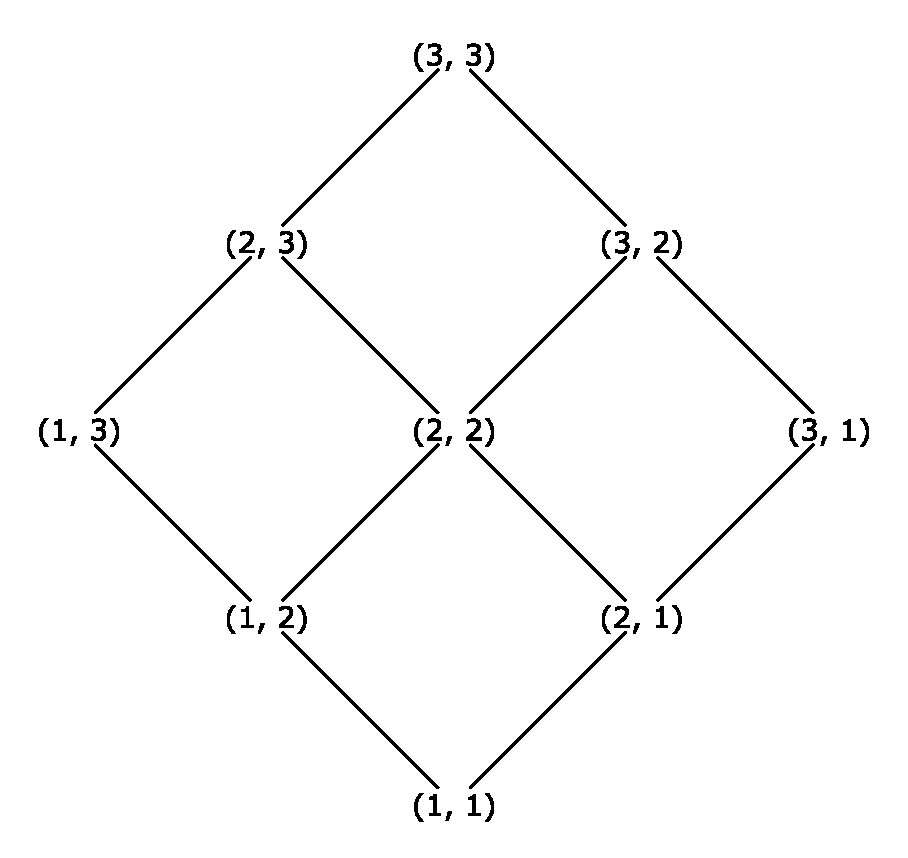
\includegraphics[width=13cm]{aufgabe1a-hasse}
%\caption{This is a figure.}
\end{center}
\end{figure}

\subsection*{b)}
Gegeben zwei Elemente $(x_1, y_1) \in \mathbb{N}^+ \times \mathbb{N}^+ $ und
$(x_2, y_2) \in \mathbb{N}^+ \times \mathbb{N}^+ $ kann das Infimum mit folgender Funktion berechnet werden:

\begin{align*}
&inf:  (\mathbb{N}^+ \times \mathbb{N}^+) \times  (\mathbb{N}^+ \times \mathbb{N}^+)  \to \mathbb{N}^+ \times \mathbb{N}^+ \\
&((x_1, y_1), (x_2, y_2))  \mapsto (min(x_1, x_2), min(y_1, y_2))
\end{align*}

Das Supremum berechnet diese Funktion:
\begin{align*}
&sup:  (\mathbb{N}^+ \times \mathbb{N}^+) \times  (\mathbb{N}^+ \times \mathbb{N}^+)  \to \mathbb{N}^+ \times \mathbb{N}^+ \\
&((x_1, y_1), (x_2, y_2))  \mapsto (max(x_1, x_2), max(y_1, y_2))
\end{align*}

\subsection*{c)}
Sei $ X \subseteq  \mathbb{N}^+ \times \mathbb{N}^+ $ und $ x \in X$. Dann lässt sich das Infimum mit folgender Funktion berechnen:
\begin{align*}
& \Inf : X \to x \\
& \Inf (X) = (min(\{x \medspace | \medspace \exists y. (x, y) \in X\}),
min(\{y \medspace| \medspace\exists x. (x, y) \in X\})
% TODO: abstände um | schöner machen
\end{align*}

Das Supremum berechnet diese Funktion:
\begin{align*}
& \Sup : X \to x \\
& \Sup (X) = (max(\{x \medspace| \medspace\exists y. (x, y) \in X\}),
max(\{y \medspace| \medspace\exists x. (x, y) \in X\})
% TODO: Abstände
\end{align*}
Für unendliche Teilmengen $X$ ist die Funktion undefiniert, da dann $max$ kein größtes Element finden kann.

\subsection*{d)}

\begin{align*}
& \bot = (0, 0)
\end{align*}
$\top $ existiert nicht, da die Trägermenge $ \mathbb{N}^+ \times \mathbb{N}^+ $ das Kreuzprodukt der natürlichen Zahlen ist.
Da $\mathbb{N} $ unendlich ist und kein größtes Element besitzt, gibt es auch in $ \mathbb{N}^+ \times \mathbb{N}^+ $ kein größtes Element.

\subsection*{e)}
$V$ ist ein Verband, da die Funktionen aus Aufgabenteil b) für jede zweielementige
 Teilmenge von $V$ das Infimum und das Supremum berechnen können.
Allerdings ist $V$ kein vollständiger Verband, da die Funktion $\Sup$ aus
Aufgabenteil c) für unendliche Teilmengen der Trägermenge undefiniert ist.
Das heißt es existiert nicht für alle Teilmengen der Trägermenge von $V$
 ein Supremum und somit kann $V$ kein vollständiger Verband sein.

\subsection*{f)}
Zu zeigen: Für alle $(x_1, y_1), (x_2, y_2) \in \mathbb{N}^+ \times \mathbb{N}^+ $ gilt: \\
$ (x_1, y_1) \leq_2 (x_2, y_2) \Rightarrow f((x_1, y_1)) \leq_2 f((x_2, y_2))$ \\
Seien $g$ und $h$ Funktionen: \\

\begin{align*}
& g: \mathbb{N}^+ \to  \mathbb{N}^+\\
&  g(x) = x! \\
& h: \mathbb{N}^+ \to  \mathbb{N}^+\\
&  h(y) = 2y^2 +2y -1 \\
\end{align*}
Es gilt offensichtlich:
\begin{align*}
& f((x, y)) = (h(y), g(x))
\end{align*}
Seien $ (x_1, y_1), (x_2, y_2) \in \mathbb{N}^+ \times \mathbb{N}^+ $
 mit $ (x_1, y_1) \leq_2 (x_2, y_2) $.
Dann gilt:

\begin{align}
& f((x_1, y_1)) = (h(y_1), g(x_1))
\end{align}

Es gilt außerdem:

\begin{align}
& f((x_2, y_2)) = (h(y_2), g(x_2))
\end{align}

Um die Prämisse zu erfüllen muss gelten:
\begin{align*}
& f((x_1, y_1)) \leq_2 f((x_2, y_2)) \\
\end{align*}
Aus (1) und (2) folgt, das folgendes ebenso gelten muss \\
\begin{align*}
& \Leftrightarrow (h(y_1), g(x_1)) \leq_2 (h(y_2), g(x_2)) \\
\end{align*}
Aus der Definition von  $\leq_2 $ folgt, dass dazu gelten muss: \\
\begin{align*}
& \Leftrightarrow h(y_1) \leq h(y_2) \land  g(x_1) \leq g(x_2) \\
\end{align*}

Betrachte beide Voraussetzungen getrennt: \\
1. Zu zeigen: $ h(y_1) \leq h(y_2) $ \\
Das gilt mit $y_1 \leq y_2$ immer, wenn $h$ monoton ist. \\
Dazu muss gelten: $h(n) \leq h (n+1), n \in \mathbb{N}^+$ \\
\begin{align*}
 h(n) &= 2n^2+2n-1 &\\
&\leq 2n^2 +6n +3 = 2n^2 +4n +2 +2n +2 -1 & n > 0\\
& = 2(n+1)^2 + 2(n+1) -1 = h(n+1) &\\
\end{align*}
Also ist $h$ monoton und die erste Voraussetzung gilt.

2. Zu zeigen: $g(x_1) \leq g(x_2) $ \\
Das gilt unter der gegebenen Voraussetzung $ x_1 \leq x_2 $ immer,
wenn $g$ monoton ist. \\
Dazu muss gelten: $g(n) \leq g(n+1), n \in \mathbb{N}^+ $ \\
\begin{align*}
g(n) &= n! &\\
&\leq (n+1) * n! & n > 0\\
& =(n+1)!= g(n+1)&
\end{align*}
Also ist auch $g$ monoton und die zweite Voraussetzung gilt ebenso.\\

Aus der Gültigkeit beider Voraussetzungen folgt, dass auch $f$ monoton ist.\\
$\Box$



%Das gilt mit $y_1 \leq y_2$ immer, wenn h monoton ist. \\
%Beweis der Monotonie von h per vollständige Induktion:\\
%Induktionsbehauptung: $\forall n \in \mathbb{N}^+. h(n) \leq h(n+1)$ \\
%Induktionsanfang $n = 1$ \\
%$ h(n) = h(1) = 2 + 2 -1 = 3 $\\
%$ h (n +1) = h(2) = 8 + 4 -1 = 11 $\\
%Damit gilt die IB für ein $ n \in \mathbb{N}$.\\
%Induktionsvoraussetzung: Es gilt $h(n) \leq h(n+1)$ \\
%Induktionsschritt: Betrachte $ n+1$ \\
%Zu zeigen: $ h(n+1) \leq h(n+1+1) $\\
%$ h(n+1) = 2(n+1)^2 + 2(n+1) -1 $ \\
%$ = 2(n+1)^2 +2n + 2 -1 = 2(n+1)^2 + 2n + 1 $\\
%$ = 2(n^2 + 2n + 1) + 2n + 1 $ \\
%$ = 2n^2 + 4n + 2+ 2n +1 $ \\
%$ = 2n^2 + 6n +3 $\\
%Mit $ n > 0 $und der IV gilt: \\
%$ \le 2n^2 + 10n + 11 $ \\
%$ = 2n^2 + 8n +8 + 2n + 4 -1 $ \\
%$ = 2(n^2 +4n+4) + 2n +4 -1 $ \\
%$= 2(n+2)^2 + 2(n+2) -1$\\
%$ = h( n + 2) = h(n+1+1)$ \\
%Somit gilt die Induktionsbehautung für ein $ n $ sowie $(n+1)$,
% also für alle $n \in \mathbb{N}^+$.
%
%
%
%2. Zu zeigen: $ g(x_1) \leq g(x_2) $\\
%Das gilt mit $ x_1 \leq x_2$ immer, wenn g monoton ist.\\
%TODO: Beweis der Monotonie von g (vollst. Induktion)
%
%Somit gelten beide Voraussetzungen und damit ist auch f monoton.\\
%$\Box $

\subsection*{Aufgabe 2 - Hennessy-Milner Logik: Formalisierung}

\subsubsection*{a)}

i) 
\begin{align*}
F_1 =& \poss{elefanten}\poss{warte 1min}\poss{warte 1min}\poss{robben}\true\\
\end{align*}

ii) 
\begin{align*}
F_2 =& \poss{robben}\poss{verlassen}\true\\
\end{align*}

iii) 
\begin{align*}
F_3 =& \necess{robben}\necess{verlassen}\false\\
\end{align*}

iv) 
\begin{align*}
F_4 =& \necess{robben}\necess{nilpferde}\false\\
\end{align*}

v) 
\begin{align*}
F_5 =& \poss{jahreskarte}\poss{känguru}\true\\
	&\lor\poss{bezahlen}\poss{kartezeigen}\poss{känguru}\true\\
\end{align*}

\subsubsection*{b)}

\begin{align*}
\denot{F_1}
	=& \{WNK\} 	& ja, da WNK \in \denot{F_1} = \{WNK\}\\
\denot{F_2}
	=& \{WE\} 	& ja, da \denot{F_5} \neq \emptyset\\
\denot{F_3}
	=& \Proc \setminus \{WE\} 	& ja, da \denot{F_5} \neq \emptyset\\
\denot{F_4}
	=& \Proc\\
\denot{F_5}
	=& \{Eingang\}
\end{align*}
 % Klammern um Inf & Sup nötig?

%\section*{Blatt 12}
\section*{Aufgabe 3: Bisimulation}

\begin{alignat*}{3}
\mathcal{F}^{1}(Proc \times Proc) &= r(s(\{&&(P_1, P_2),(P_1, P_5),(P_1, Q_1), (P_1, Q_2),(P_2, P_5),(P_2, Q_1),\\
								  &		  &&(P_2, Q_2),(P_3, Q_3),(P_4, Q_4),(P_5, Q_2),(P_5, Q_1),(Q_1, Q_2)\}))
\end{alignat*}
\\
$\mathcal{F}^{2}(Proc \times Proc) = r(s(\{(P_1, P_5),(P_1, Q_1),(P_2, Q_2),(P_3, Q_3),(P_5, Q_1)\}))$
\\
$\mathcal{F}^{3}(Proc \times Proc) = r(s(\{(P_2, Q_2),(P_5, Q_1)\}))$
\\
$\mathcal{F}^{4}(Proc \times Proc) = r(s(\{(P_5, Q_1)\}))$
\\
$\mathcal{F}^{5}(Proc \times Proc) = r(s(\{(P_5, Q_1)\}))$
\\\\
Da $\mathcal{F}^{4} = \mathcal{F}^{5}$ sind beide ein Fixpunkt.
\\
Somit erhalten wir, dass $P_5$ und $Q_1$ das einzige nicht trivial bisimilare Paar ist. Es gilt $P_5$ \bisim $Q_1$

\section*{Aufgabe 4: Bisimulation (2)}

$\mathcal{F}^{1}(Proc \times Proc) = r(s(\{(R_1, R_7),(R_2, R_4),(R_2, R_6),(R_3, R_5),(R_4, R_6),(R_8, R_9)\}))$
\\
$\mathcal{F}^{2}(Proc \times Proc) = r(s(\{(R_2, R_6),(R_3, R_5)\}))$
\\
$\mathcal{F}^{3}(Proc \times Proc) = r(s(\{(R_2, R_6),(R_3, R_5)\})) = \mathcal{F}^{2}$
\\\\
Da $\mathcal{F}^{2} = \mathcal{F}^{3}$ sind beide ein Fixpunkt.
\\
Somit erhalten wir, dass $R_2$ und $R_6$ sowie $R_3$ und $R_5$ die einzigen nicht trivialen bisimilaren Paare sind. Es gilt $R_2$ \bisim $R_6$ und $R_3$ \bisim $R_5$.


\end{document}
